\chapter{Implementation}
This chapter deals with the implementation details of the campus app. It starts by describing the process for the collection and processing of geodata and explains how the campus map and the navigation system are derived from it. It further showcases the procedure for gathering campus-relevant data from publicly available web sources and concludes with a description of the implementation process for the user interface, which finally merges the campus map, navigation and information layers.

\label{cha:implementation}
\section{Collection of geodata and POI}
Geodata refers to all data about geographic information. In the case of this thesis, it mainly consists of coordinate points, which describe certain campus-relevant entities, such as outlines of buildings, the street network, pathways, entrances as well as boundaries of green areas and water. Except for single-point usage, multiple coordinate points can be grouped into polygons, representing the closed outline of an entity and polylines, mainly used to describe lines, streets and paths. In addition to its coordinates, geodata also describes other attributes of an entity e.g., its name, altitude, width or height. This can be used for tasks like geocoding/reverse geocoding, display of information, 3d terrain generation or general data analysis.

\subsection{Overview of needed geodata}
Geodata is the building block for map generation and routing through a street network. The following list presents an overview of the geodata needed for this implementation:

\begin{itemize}
    \item Buildings: The outlines of buildings are polygons consisting of multiple coordinate points. Additionally to that, the height of each building is needed for appropriate 3D representation.
    \item Streets: Streets are represented by polylines and are (based on their importance, size and purpose) divided into three categories, namely main roads, small roads and pathways. This separation allows the different road types to be designed and displayed independently from each other. They can therefore vary in size, style and coloring when used in the campus map.
    \item Green areas: The outlines of green areas are retrieved in the polygon format.
    \item Water: The outlines of water (especially rivers) are also retrieved in the polygon format.
    \item Entrances to TU Berlin's buildings: To successfully connect TU Berlin's buildings to its underlying street network, entrances need to be defined. A single-point representation paired with an identifier for the buildings is used.
\end{itemize}

\subsection{Collection data from OSM via Overpass Turbo API}
OpenStreetMap (OSM) is a free mapping service, that allows its users to access, edit and download its available geodata. Its main querying language is Overpass Turbo which comes with a web interface for data mining and a respective web API \cite{openstreetmap_overpass_turbo}. This querying system is used to provide a starting point for the complete set of geodata needed for this thesis. The used bounding box for retrieval is (52.49993096650543, 13.307022255971093) for the south-west and (52.52269751545147, 13.341918533901309) for the north-east corner. The following table presents the queried data over all categories together with the node count (one node usually consists of a coordinate point), the type of retrieved data and the respective query.

\begin{table}[!ht]
	\small
	\centering
	\begin{tabular}{|l|l|l|l|}
		\hline
		Entities                & Type of geodata       & Number of queried nodes       & Overpass Turbo query \\
		\hline
        Buildings               & Polygons              & 1949                          & \ref{buildings} \\
		\hline
		Main roads              & Polylines             & 2036                          & \ref{main_roads} \\
		\hline
		Small roads             & Polylines             & 2578                          & \ref{small_roads} \\
		\hline
		Pathways and sidewalks  & Polylines             & 11757                         & \ref{pathways} \\
		\hline
        Green areas             & Polygons              & 5057                          & \ref{green_areas} \\
		\hline
        Water                   & Polygons              & 1651                          & \ref{water} \\
		\hline
        Entrances               & Single points         & 1758                          & \ref{entrances} \\
		\hline
	\end{tabular}
	\caption{Overview of queried geodata}
\end{table}

This results in a total of 26786 queried nodes. Each category is further exported as a separate geoJSON file, containing the relations between individual points (polygon, polyline, single node) as well as other OSM attributes (e.g., the names of buildings and streets, the height of buildings, etc.).

\subsection{Correction of OSM data for map generation in QGIS}
Since the queried data contains several imperfections that are not desirable for map generation, all geoJSON files are imported into QGIS for cleanup. QGIS is an open-source geographic information system, that provides a convenient visual user interface for editing geodata. The following images present a visual reference for the changes performed to the data (note, that all street data is represented in one image for simplicity and that water data does not need cleanup and is therefore not present).

\begin{figure}[H]
	\centering
	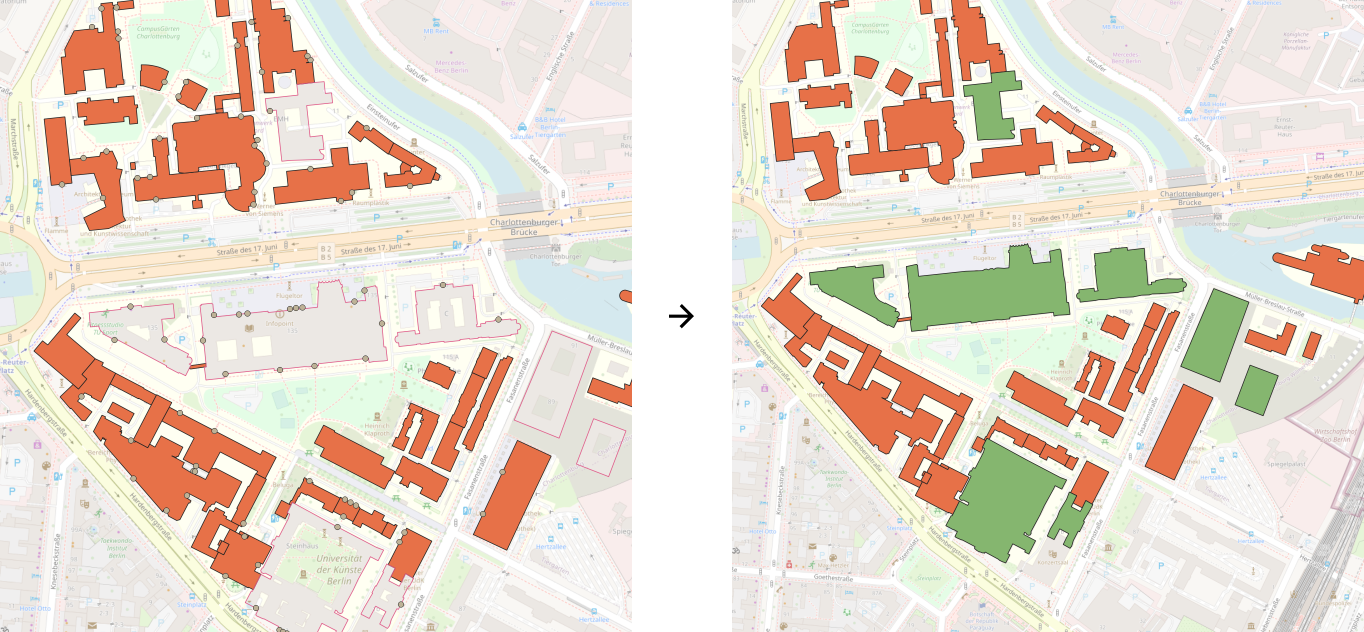
\includegraphics[width=0.65\textwidth]{images/preparing_buildings.png}\\
	\caption{Correction of TU Berlin's building data}
\end{figure}

\begin{figure}[H]
	\centering
	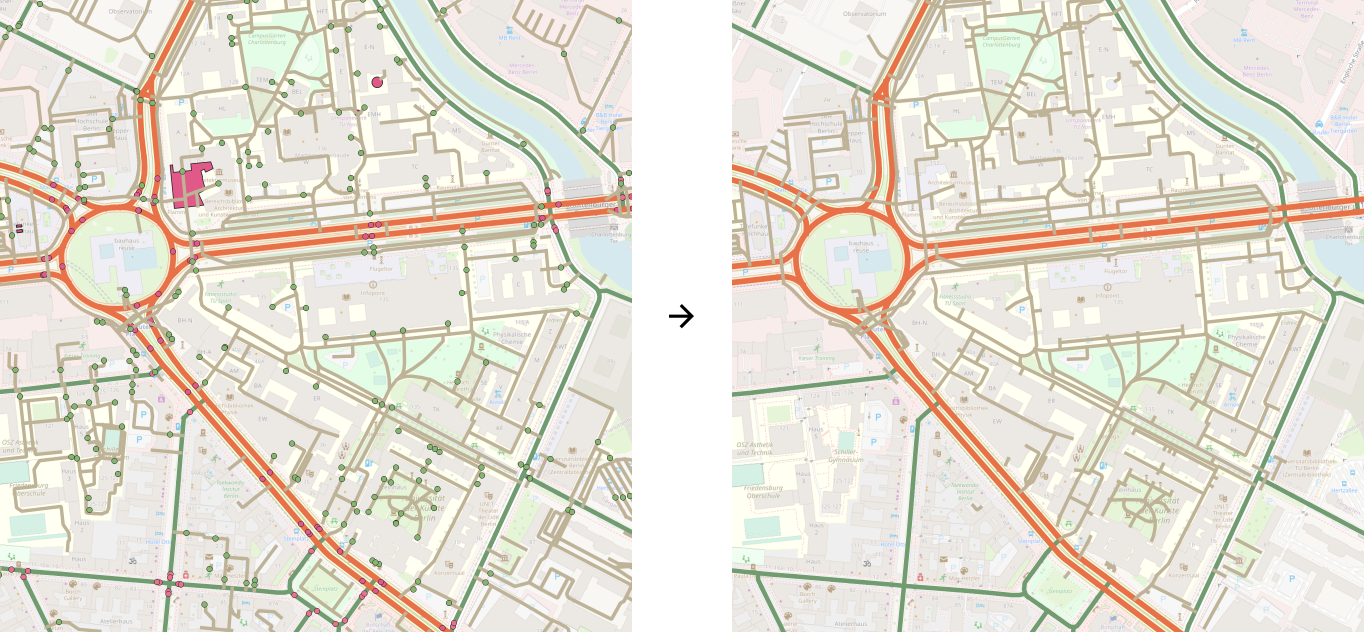
\includegraphics[width=0.65\textwidth]{images/preparing_streets.png}\\
	\caption{Correction of TU Berlin's street network data}
\end{figure}

\begin{figure}[H]
	\centering
	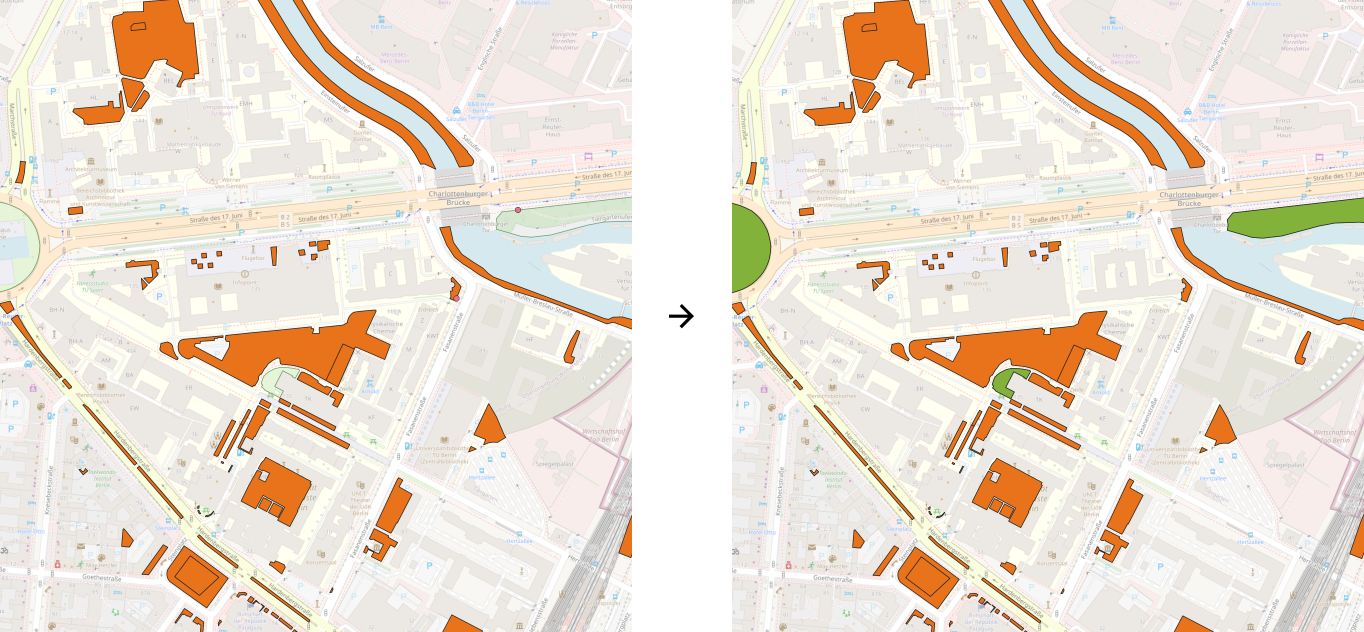
\includegraphics[width=0.65\textwidth]{images/preparing_green_areas.png}\\
	\caption{Correction of TU Berlin's green area data}
\end{figure}

\begin{figure}[H]
	\centering
	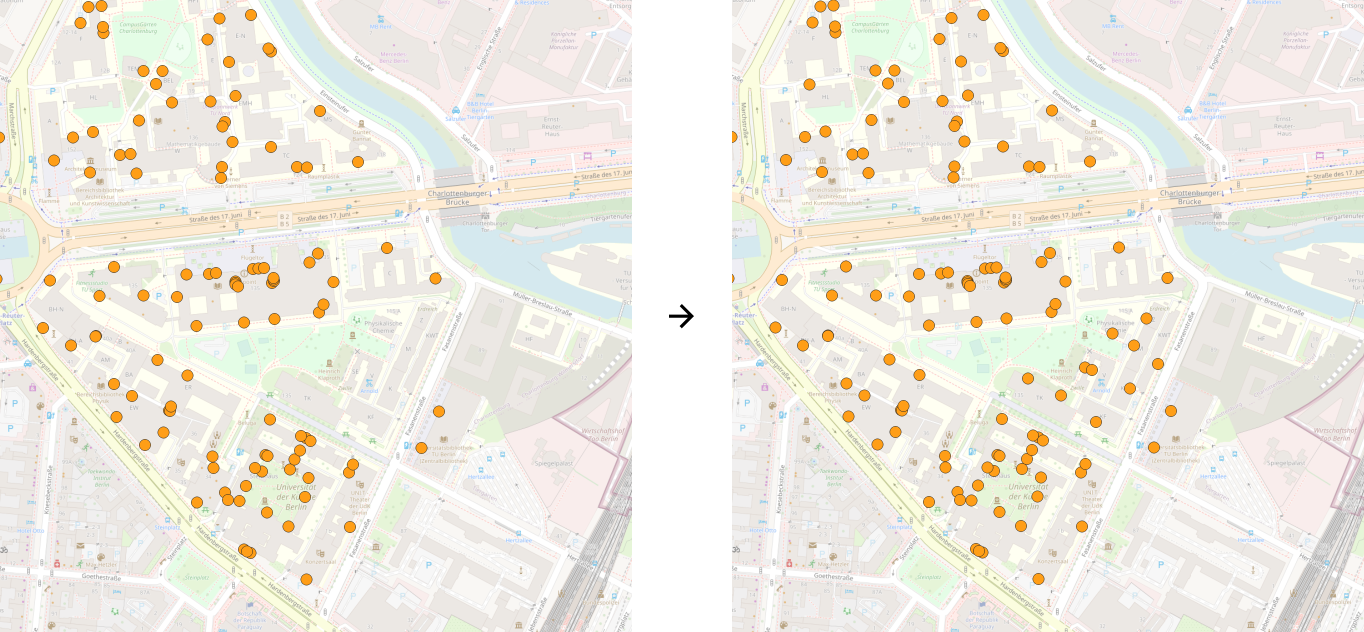
\includegraphics[width=0.65\textwidth]{images/preparing_entrances.png}\\
	\caption{Correction of TU Berlin's entrance data}
\end{figure}

The main problem that gets corrected consists of wrong geometry types in the data. Since is desirable that every dataset only contains one kind of geometry (e.g., the data for the buildings should only contain polygon outlines, the street data should only contain polylines, etc.), all wrong geometry types in a dataset are either deleted (e.g., single points in the street or building data) or reshaped to match the expected geometry type (e.g., polylines representing the outline of a building/green area are converted into polygons).

Missing entities (e.g., certain entrances to buildings) are furthermore added and information not related to the campus (mainly data from the street network) is removed.

\section{Generation of digital campus map}
This section provides a detailed overview of the procedure for generating the digital campus map in the Unity3d real-time rendering engine. It starts by describing how the already collected data is used and imported into Unity and further explains how 3d entities are created from it. The section concludes with a brief overview of the map design and the implementation details for common map gestures such as pinch-to-zoom or slide-to-move.

\subsection{Data import and conversion in Unity}
The first step in the map generation process is the import of the manually corrected OSM data from QGIS into Unity3d. This is done in geoJSON format \cite{geoJSON}, which specifies a certain JSON structure for geodata and contains all coordinate points and their relations to each other as well as additional attributes.

After import, a C\# class named GeoNode is introduced, which represents a single node in the OSM data and contains its position. Furthermore, a class for every category of entities on the campus map (buildings, green areas, streets, ...) is implemented, which contains an array of position vectors, derived from the GeoNodes, describing the respective (out)line of its entity. Lastly, methods for parsing geoJSON into their C\# object representations are created.

One main problem during the parsing process is the fact that OSM and the campus map are constructed differently: While OpenStreetMap consists of a map projected onto a sphere, the campus map is generated on a 2-dimensional plane. This results in the usage of different coordinate systems. OpenStreetMap in this case uses the WGS 84/Pseudo-Mercator system \cite{pseudo_mercator_1} \cite{pseudo_mercator_2}, which describes points on Earth as pairs of latitude and longitude. This is ideal for spherical map projection but is not suitable for a 2d plane base, where general length units (e.g., meters) are advantageous. A conversion from WGS 84/Pseudo-Mercator to 2d position vectors (x, y) in meters from the map origin is therefore chosen and integrated into the parsing process. It is further defined that x represents the longitude and y is the original latitude component of WGS 84.

The unit conversion process is based on OpenStreetMap's reference implementation of the WGS 84/Pseudo-Mercator projection \cite{mercator_projection_implementation} in C and computes the following formulas:

\[x(lon) = lon * r\]
\[y(lat) = \ln(\tan(\frac{lat}{2} + \frac{\pi}{4})) * r\]

Where the WGS 84/Pseudo-Mercator coordinates (lat, lon) in radians are converted to (x, y) in approximate meters, with r being the radius of the Earth (note that the WGS 84 coordinates are usually defined in degrees and need to be converted into radians beforehand).

The resulting coordinates are furthermore stored inside the GeoNode class as floats and are also converted into Unity's 3-dimensional Vector3 position system, where a position (x, y) is mapped to Vector3(x, 0, y). To center the campus section of TU Berlin around Unity's origin at Vector3(0, 0, 0), the central map point of campus Charlottenburg (52.5126624, 13.3231489) is subtracted from all OSM data points before conversion.

\subsection{Mesh generation for streets, green areas, water and 3d buildings}
Meshes are the building blocks for every 3-dimensional object rendered on a digital screen. They define the structure of an object and provide parameters for lighting calculations and material mapping and are generated by defining a set of attributes, the most relevant ones being:

\begin{enumerate}
	\item Vertices: Vertices are points in space, that define the corners of an object.
	\item Triangles: To generate a surface area, 3 different previously defined vertices are connected to form a triangle. A net of triangles finally determines the final shape and surface of an object. One important concept to keep in mind is the backface culling step of the render pipeline: For optimization purposes, the rendering engine decides whether surfaces created by triangles are drawn or not by using the order of vertices that define a certain triangle. Unity3d only renders triangles with a clockwise ordering of vertices when projected onto the screen. The whole process of generating a triangle net to fill a predefined surface area is called surface triangulation.
	\item Surface normals: Surface normals are vectors that are perpendicular to their related surface. They are used to differentiate between the "front" and "back" sides of their respective surface and are an important component for calculating the lighting of an object. Generally, each triangle is assigned a surface normal, which can be calculated by taking the cross product of two different edges. (Note: Unity differs from that and uses a surface normal per vertex approach. This normal can be calculated by averaging all normals of triangles containing the respective vertex. For better understanding, the normal per triangle model is nevertheless displayed in the figures.)
	\item UV coordinates: UVs are 2-dimensional coordinates that specify the texture mapping of an object. There are as many UV coordinates as vertices in a mesh. Based on the shape of an object, the UV coordinate system can be mapped differently onto the vertices.
\end{enumerate}

\begin{figure}[H]
	\centering
	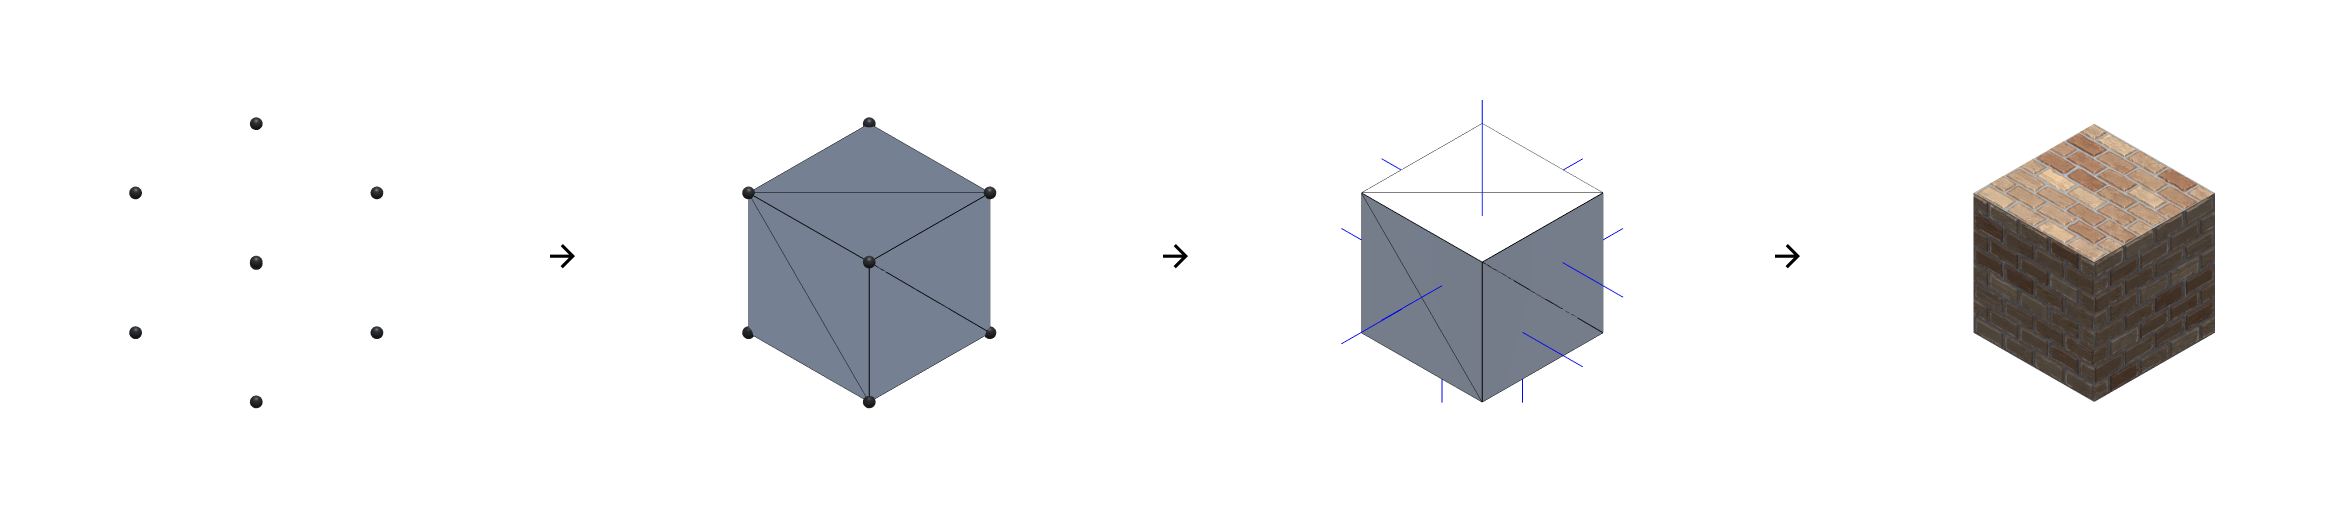
\includegraphics[width=0.8\textwidth]{images/mesh_generation_process.png}\\
	\caption{Mesh generation process for a cube}
\end{figure}

In the case of the campus map, several simplifications can be made: Surface normals can be calculated from the predefined vertices and triangles. Since the entities on the campus are only unicolored (no distortable textures are applied) the 2-dimensional UV coordinates can be chosen arbitrarily (or not at all) for every vertex. This breaks down the mesh generation process for the campus map into two separate tasks: Defining the outlining vertices of an entity from its GeoNodes and triangulating its corresponding surface.

Mesh generation for streets: To define the outline of a street, the corresponding GeoNodes, which only represent a polyline, need to be replaced by two separate polylines defining the edges of the street. The width $w$ of the street is then defined by the distance between both outlining polylines. To generate them, every GeoNode at index $i$ with coordinate $\vec{g_{i}}$ of the original polyline can be shifted with a vector $\vec{v}$, which is perpendicular to the road direction at $\vec{g_{i}}$ and the up-facing vector (in the case of Unity Vector3(0, 1, 0)). A pair of outlining points can be therefore generated for every GeoNode coordinate $\vec{g_{i}}$:

\[\vec{eRight_{i}} = (\vec{g_{i + 1}} - \vec{g_{i}}) \times (0, 1, 0) * \frac{w}{2}\]

\[\vec{eLeft_{i}} = (\vec{g_{i + 1}} - \vec{g_{i}}) \times (0, 1, 0) * - \frac{w}{2}\]

Where $\vec{eRight_{i}}$ is the point on the right polyline and $\vec{eLeft_{i}}$ is the point on the left polyline corresponding to $\vec{g_{i}}$ (when looked into the direction $\vec{g_{i + 1}} - \vec{g_{i}}$).

These vertices can be further triangulated by grouping 4 points. To fill the street surface between coordinates $\vec{g_{i}}$ and $\vec{g_{i + 1}}$, the points $A = \vec{eLeft_{i}}$, $B = \vec{eRight_{i}}$, $C = \vec{eRight_{i + 1}}$ and $D = \vec{eLeft_{i + 1}}$ are selected and two triangles $ACB$ and $ADC$ are created.

\begin{figure}[H]
	\centering
	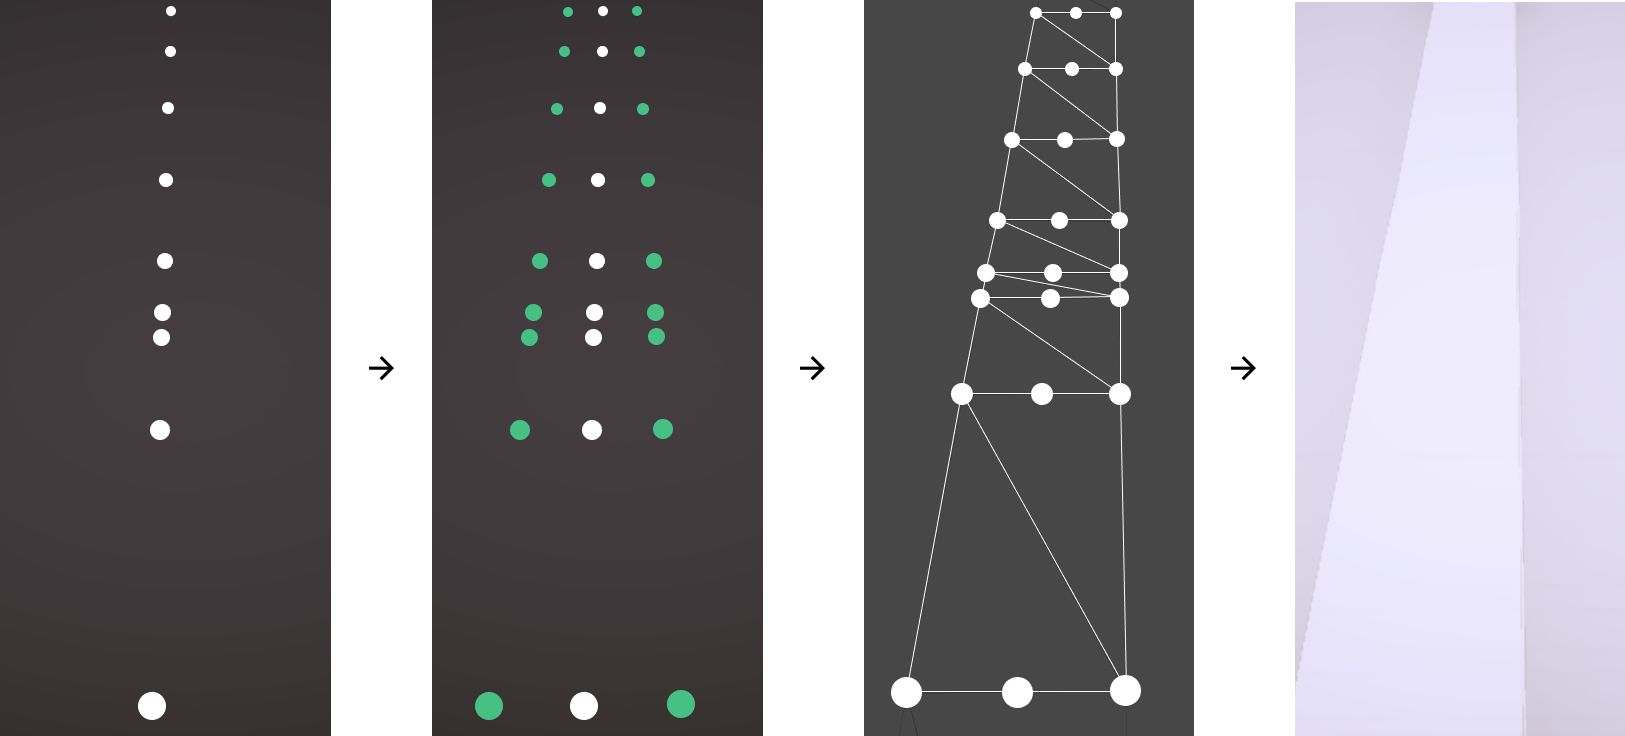
\includegraphics[width=0.8\textwidth]{images/street_mesh_generation.png}\\
	\caption{Mesh generation process for a street}
\end{figure}

Mesh generation for buildings: Buildings consist of a ceiling tile and a set of surrounding walls. To determine the outlining vertices, the predefined set of GeoNode coordinates can be extended by shifting it upwards. The amount of shift is determined by the height $h$ of the respective building. For every GeoNode coordinate $\vec{g_{i}}$, a new coordinate $\vec{c_{i}}$ is therefore created and added to the final set of building vertices:

\[\vec{c_{i}} = \vec{g_{i}} + (0, 1, 0) * h\]

The triangulation process for the resulting set of vertices can be broken down into two separate procedures for the ceiling and the walls. On the one hand, a routine similar to the street triangulation process can be applied to create the walls. A single wall is here defined by two consecutive GeoNode coordinates $\vec{g_{i}}$ and $\vec{g_{i + 1}}$ and their corresponding shifted coordinates $\vec{c_{i}}$ and $\vec{c_{i + 1}}$. The surface area between these four points is then exactly triangulated like a piece of street defined by four points (see the previous section).

On the other hand is the triangulation process for the ceiling tile. In this case, a standard algorithm for the triangulation of concave polygons can be applied. The "Triangulation by Ear Clipping" \cite{triangulation_by_ear_clipping} algorithm is used with a C\# implementation for Unity derived from \cite{triangulation_unity_library}. To avoid backface culling problems and for simplicity, all triangles are generated double-sided, with vertices specified in both orderings.

\begin{figure}[H]
	\centering
	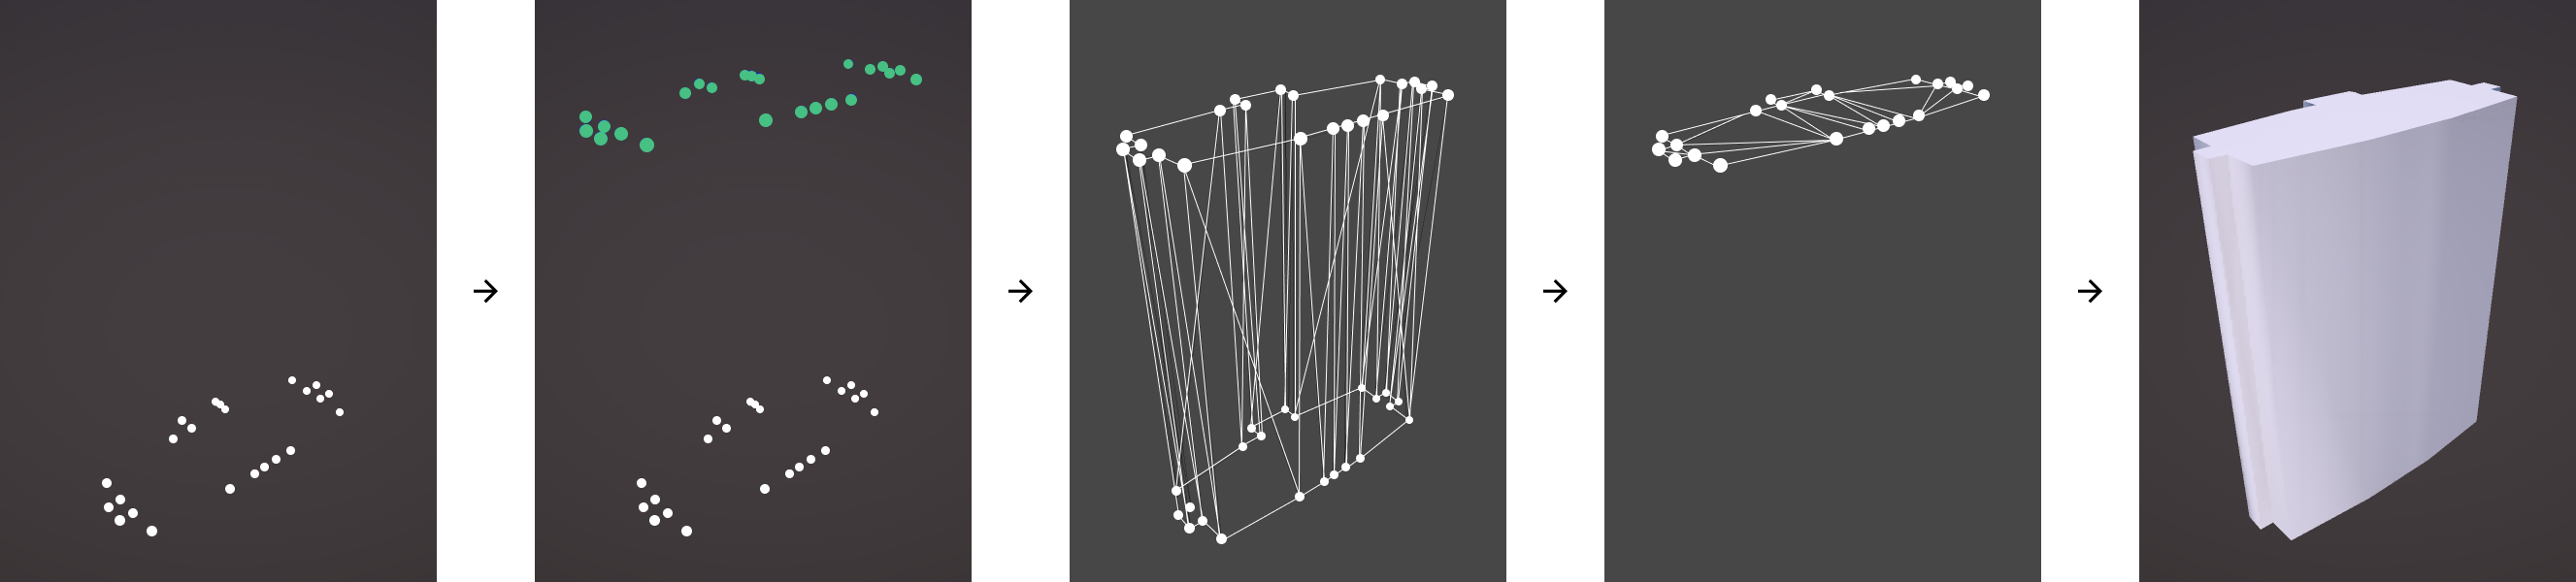
\includegraphics[width=0.8\textwidth]{images/building_mesh_generation.png}\\
	\caption{Mesh generation process for a building}
\end{figure}

Mesh generation for green areas and water: Since green areas and water both consist of flat and concave polygons, the same procedure can be used for generating both respective meshes. The outlining vertices are in this case simply the predefined GeoNode coordinates and can be triangulated in the same manner as the ceiling of a building.

\subsection{Map design}
Test.
\subsection{Implementing common interaction gestures}
Test.

\section{Navigation system development}
\subsection{Representation of geodata for navigation}
\subsection{Manual generation of TU Berlin's street network}
\subsection{Routing across the campus}
\subsection{Time estimation for routes}
\subsection{Embedding the current user location via GPS}

\section{Interactive information layer development}
\subsection{Collection of campus relevant information from the web}
\subsection{Processing of information and internal representation}

\section{User interface development}
\subsection{Navigation system}
\subsection{Information layer}
\subsection{Enhancing the user experience with additional screens and features}